\documentclass[]{article}

% Imports the catppuccin theme, using the mocha flavor,
% from the directory above. Actual implementation
% wouldn't need the import package unless the theme
% and the document are in different directories.
\usepackage{import}
\usepackage{xcolor}
% \usepackage{fancyhdr}
\usepackage{cancel}
\usepackage{mathtools}

% For permutations and combinations
\newcommand\Myperm[2][^n]{\prescript{#1\mkern-2.5mu}{}P_{#2}}
\newcommand\Mycomb[2]{\prescript{#1\mkern-0.5mu}{}C_{#2}}

% Colors
\definecolor{yorhabg}{HTML}{FFFFFF}
\definecolor{yorhafg}{HTML}{000000}
\definecolor{yorhagrid}{HTML}{B5AF9C}
\definecolor{mred}{HTML}{D67069}
\definecolor{mblue}{HTML}{6887A1}

\pagecolor{yorhabg}
\color{yorhafg}

\usepackage{preamble}

% Removes padding above title
\usepackage{titling}
\setlength{\droptitle}{-10em}

% Font package
\usepackage[T1]{fontenc}

\usepackage{fouriernc}

\usepackage{sectsty}
\usepackage{graphicx}
\usepackage{amsmath}
\usepackage{amsfonts}
\usepackage{amssymb}
\usepackage{tikz}
\usepackage{pgfplots}
\pgfplotsset{compat=1.18}
\usepackage[skins, most]{tcolorbox}
\usepackage{enumitem}

\DeclareMathOperator{\sgn}{sgn}

\usepackage{tikz}
\usepackage{eso-pic}
\usetikzlibrary{calc,shadows.blur}
\usetikzlibrary{angles, quotes}
\usetikzlibrary{3d}

% Margins
\topmargin=0in
\evensidemargin=0in
\oddsidemargin=0in
\textwidth=6.5in
\textheight=9.0in
\headsep=0.25in

\AtBeginEnvironment{tcolorbox}{\small}

\newtcolorbox{imp}{enhanced,arc=0mm,colback=yorhabg,colframe=mred,leftrule=10mm,coltext=yorhafg,%
overlay={\node[anchor=west,outer sep=2pt] at (frame.west) {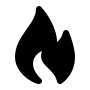
\includegraphics[width=6mm]{images/imageb.png}}; }}

\newtcolorbox{shortcut}{enhanced,arc=0mm,colback=yorhabg,colframe=mred,leftrule=10mm,coltext=yorhafg, coltitle=yorhabg, title=\texttt{Shortcut.}, 
overlay={\node[anchor=west,outer sep=2pt] at (frame.west) {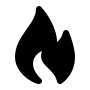
\includegraphics[width=6mm]{images/imageb.png}}; }}

\newtcolorbox{question}[1]{
    enhanced, 
    colback=yorhabg,
    colframe=mblue,
    coltext=yorhafg,
    coltitle=yorhabg,
    attach boxed title to top left={yshift*=-\tcboxedtitleheight}, 
    title=\texttt{#1},
    boxed title size=title,
    boxed title style={%
        rounded corners=northeast, 
        rounded corners=northwest, 
        colback=tcbcolframe, 
        boxrule=0pt,
    },
    underlay boxed title={%
        \path[fill=tcbcolframe] (title.south west)--(title.south east) 
            to[out=0, in=180] ([xshift=5mm]title.east)--
            (title.center-|frame.east)
            [rounded corners=5pt] |- 
            (frame.north) -| cycle; 
    },
}

\newcommand\bb[1]{\textcolor{yorhafg}{\textbf{#1}}}

\title{\textbf{MATA31 - Assignment \#5}}
\author{Satyajit Datta \ 1012033336}
\date{\today}

\begin{document}

\maketitle

\section{Textbook Questions}

\begin{question}{1.3.62}
    Prove.
    \[
    \lim_{x\to -2^-} \frac{1}{x+2} = -\infty
    \]
\end{question}
Want to show: 
\[
    \forall M < 0\;\exists\; \delta>0 \quad \text{s.t} \quad 
    0 < -2-x < \delta \Longrightarrow \frac{1}{x+2} < M
\]

\underline{\bf{Proof.}}

\underline{Let} $M < 0$ be arbitrary.

\medbreak

\underline{Choose} $\delta = -\frac{1}{M}$. Note $\delta > 0$.

\medbreak

\underline{Assume} $0 < -2-x < \delta$. Then, 

\begin{align*}
0 < -2 - x < \delta &\implies -2 - x < -\frac{1}{M} 
    && \text{(by our choice of $\delta$)} \\[2mm]
&\implies x + 2 > \frac{1}{M} 
    && \text{(because $x < -2$)} \\[2mm]
&\implies \frac{1}{x+2} < M
    && \text{(by properties of inequalities)}
\end{align*}

As required to prove. $\blacksquare$

\begin{question}{1.3.64}
    Prove.
    \[
    \lim_{x\to -\infty} \frac{2x-1}{x} = 2
    \]
\end{question}

Want to show: 
\[
    \forall \varepsilon > 0\;\exists\; N<0 \quad \text{s.t} \quad 
    x < N \Longrightarrow |\frac{2x-1}{x}-2| < \varepsilon
\]

\underline{\bf{Proof.}}

\underline{Let} $\varepsilon > 0$ be arbitrary.

\medbreak

\underline{Choose} $N = -\frac{1}{\varepsilon}$. Note $N < 0$.

\medbreak

\underline{Assume} $x < N$. Then, 

\begin{align*}
    |\frac{2x-1}{x}-2| &= |\frac{2x-1 -2x}{x}| 
        && \text{(by algebra)} \\[6pt]
    &= |\frac{-1}{x}| 
        && \text{(by algebra)} \\[6pt]
    &= \frac{1}{|x|} 
        && \text{(by properties of $|\cdot|$)} \\[6pt]
    &= \frac{1}{-x} 
        && \text{(since $x<0$)} \\[6pt]
    \frac{1}{-x} &< \frac{1}{-N} 
        && \text{(since $x < N < 0 \implies -x > -N > 0$)} \\[6pt]
    &= \frac{1}{-(\frac{-1}{\varepsilon})} 
        && \text{(by our choice of $N$)} \\[6pt]
    &= \frac{1}{\frac{1}{\varepsilon}}
        && \text{(by algebra)} \\[6pt]
    &= \varepsilon
        && \text{(by algebra)} \\[6pt]
\end{align*}

As required to prove. $\blacksquare$
\begin{question}{1.3.66}
    Prove.
    \[
    \lim_{x\to -\infty} (3x-5) = -\infty
    \]
\end{question}
Want to show: 
\[
    \forall M < 0\;\exists\; N<0 \quad \text{s.t} \quad 
    x < N \Longrightarrow 3x-5 < M
\]

\underline{\bf{Proof.}}

\underline{Let} $M < 0$ be arbitrary.

\medbreak

\underline{Choose} $N = \frac{M}{3}$. Note $N < 0$.

\medbreak

\underline{Assume} $x < N$. Then, 

\begin{align*}
x < N &\implies x < \frac{M}{3} 
    && \text{(by our choice of $N$)} \\[2mm]
&\implies 3x < M 
    && \text{(by algebra)} \\[2mm]
&\implies 3x - 5 < M - 5
    && \text{(by algebra)}\\[2mm]
&\implies 3x - 5 < M - 5 < M
    && \text{(by algebra)}\\[2mm]
&\implies 3x - 5 <  M
    && \text{(by properties of inequalities)}\\[2mm]
\end{align*}

As required to prove. $\blacksquare$
\begin{question}{1.3.70}
    Prove.
    \[
    \lim_{x\to 1} (x^2-6x+7) = 2
    \]
\end{question}

Want to show: 
\[
    \forall \varepsilon > 0\;\exists\;\delta >0 \quad \text{s.t} \quad 
    0 < |x-1| < \delta \Longrightarrow |(x^2-6x+7)-2| < \varepsilon
\]

\underline{\bf{Proof.}}

\underline{Let} $\varepsilon > 0$ be arbitrary

\medbreak

\underline{Choose} $\delta = \min\{5, \frac{\epsilon}{9}\} $. Note that $\delta$ > 0.

\medbreak

\underline{Assume} $0 < |x-1| < \delta$.
\medbreak
Since $x^2-6x+7-2 = (x-1)(x-5)$ and $x-1 < \delta$, we first need to obtain a bound on $|x-5|$. Then
\begin{align*}
    |x-1| < \delta &\Longrightarrow |x-1|<5
        && \text{(since $\delta = \min\{ 5, \frac{\varepsilon}{9} \} \le 5$)} \\[6pt]
    &\Longrightarrow -5 < x-1 < 5
        && \text{(by properties of $|\cdot|$)} \\[6pt]
    &\Longrightarrow -9 < x-5 < 1 
        && \text{(by algebra)} \\[6pt]
    &\Longrightarrow -9 < x-5 < 9
        &&\text{(by properties of inequalities)} \\[6pt]
    &\Longrightarrow |x-5| < 9
        &&\text{(by properties of $|\cdot|$)} \\[6pt]
\end{align*}

Therefore, $|x-5| < 9$ $(\star)$.

It now follows that:
\begin{align*}
    |x^2-6x+5| &= |(x-5)(x-1)| 
        && \text{(by algebra)} \\[6pt]
    &= |x-5||x-1| 
        && \text{(by properties of $|\cdot|$)} \\[6pt]
    &< |x-5|\delta
        && \text{(by assumption)} \\[6pt]
    &< 9\delta
        && \text{(by ($\star$))} \\[6pt]
    &= 9\frac{\varepsilon}{9} 
        && \text{(by our choice of $\delta$)} \\[6pt]
    &= \varepsilon 
        && \text{(by algebra).}
\end{align*}
As required to prove. $\blacksquare$

\begin{question}{1.4.48}
    Use graphs to determine if $f$ is continuous at the given point $x = c$.
    \[
        f(x) = \begin{cases*}
            x^2-3, \quad \text{if } x \text{ rational} \\
            3x+1, \quad \text{if } x \text{ irrational} \\
        \end{cases*}
    \]
    $c = 4$.
\end{question}
The informal definition of continuity is:
\begin{center}
    \begin{enumerate}[label=(\arabic*)]
        \item $f(c)$ exists.
        \item $\displaystyle \lim_{x\rightarrow c} f(x)$ exists.
        \item $\displaystyle \lim_{x\rightarrow c} f(x) = f(c)$
    \end{enumerate}
\end{center}

Since $c = 4 \implies c \in \mathbb{Q}$, then $f(4) = 4^2 - 3 = 16 - 3 = 13.$
Therefore, $f(c)$ exists, meaning (1) holds.
\medbreak
There are infinite irrational numbers between every rational number, therefore
we check if the limit of both pieces of the function are equal to each other. 

\[
    \lim_{x-4}\;(x^2 - 3) = 16-3 = 13.
\]

\[
    \lim_{x-4}\; (3(4) - 1) = 12+1 = 13
\]
Note that we can simply substitute c into these equations because they are both polynomials with non-negative
exponents.
\medbreak
Therfore, since $\displaystyle \lim_{x\rightarrow c} f(x)$ exists. and 
$\displaystyle \lim_{x\rightarrow c} f(x) = f(c)$, the function is continuous at 
$x = 4$.
\begin{center}
\begin{tikzpicture}
\begin{axis}[
    axis lines=middle,
    xlabel={$x$},
    ylabel={$y$},
    grid=both,
    xmin=-4, xmax=4,
    ymin=-5, ymax=10,
    samples=200,
    legend style={at={(0.97,0.03)},anchor=south east}
]
\addplot[domain=-3:3, thick, red]{x^2 - 3};
\addlegendentry{$y = x^2 - 3$}

\addplot[domain=-3:3, thick, blue]{3*x + 1};
\addlegendentry{$y = 3x + 1$}
\end{axis}
\end{tikzpicture}
\end{center}
\section{Assignment Questions}
\begin{question}{D}
    Find the supremum and infimum of the following sets, if they exist.
    \begin{center}
        \begin{enumerate}[label=(\alph*)]
            \item $A = \{\frac{1}{n} : n \in \mathbb{Z} \quad \text{and} \quad n \ne 0\}$
            \item $B = \{x \in \mathbb{Q}: 0 \le x \le \sqrt{2}\}$
            \item $C = \{x \in \mathbb{R}: x^2 + x + 1 \ge 0\}$
        \end{enumerate}
    \end{center}
\end{question}

(a). $A = \{\frac{1}{n} : n \in \mathbb{Z} \quad \text{and} \quad n \ne 0\}$

As $n \to -\infty, \frac{1}{n} \to 0^-$
As $n \to \infty, \frac{1}{n} \to 0^+$
Since $n \in \mathbb{Z}$ the biggest positive and biggest negative numbers we can obtain
are -1 and 1. Therefore, the highest number we can achieve is 1, the lowest is -1.

Therefore, the supremum is $1$, and the infimum is $-1$.
\vspace{0.1in}
\hrule
\vspace{0.1in}
(b). $B = \{x \in \mathbb{Q}: 0 \le x \le \sqrt{2}\}$

The lowest number in this set is 0, making it the infimum. There are infinitely many
rational numbers in $[0, \sqrt{2}]$, meaning that there is no biggest rational number in this set.
Therefore, the infimum is $\sqrt{2}$.
\vspace{0.1in}
\hrule
\vspace{0.1in}

(c). $C = \{x \in \mathbb{R}: x^2 + x + 1 \ge 0\}$

\[
    \Delta = 1^2 - 4(1)(1) = -3
\]

Since the discriminant $< 0$, the function does not touch the x-axis. Also, since $a > 0$, the parabola is entirely above the x-axis, 
making this set contain all real numbers. Therefore, there is no
upper or lower bound, which in turn means there is no supremum or infimum.

\begin{question}{E}
     Let $S$ be a non-empty subset of $\mathbb{R}$, and let $\alpha \in \mathbb{R}$ be an upper bound
for $S$. Prove that $\alpha$ is the supremum of $S$ if and only if for every $\varepsilon > 0$,
there exists $x \in S$ such that $x > \alpha - \varepsilon$.

Formulate an analogous characterisation of the infimum.
\end{question}

Want to show:
\[
    \alpha = \sup(S) \iff \forall \varepsilon > 0, \exists x \in S \quad \text{s.t} \quad x > \alpha - \varepsilon
\]
\underline{\textbf{Proof.}}  

\medskip

\noindent \textbf{($\Rightarrow$)}  
Assume $\alpha = \sup(S)$.  

Then, by definition, $\alpha$ is the smallest possible upper bound of $S$.

Assume $\varepsilon > 0$. Then $\alpha - \varepsilon < \alpha$. 

However, since $\alpha$ is the smallest possible upper bound, then $\alpha - \varepsilon$ is not an upper bound. In turn, this means that
$\exists x \in S \quad \text{s.t} \quad x > \alpha - \varepsilon$


\medskip

\noindent \textbf{($\Leftarrow$)}  
Solve by contradiction.

Suppose that $\forall\varepsilon>0,\exists x \in S \quad \text{s.t} \quad x > \alpha - \varepsilon$,

For sake of contradiction, assume that $\alpha \ne \sup(S)$

Then, there exists a $b$ such that b is also an upper bound of $S$, and $b \le \alpha$.

Choose $\varepsilon = \alpha - b$

Then, 
\begin{align*}
    &\exists x \in S \quad \text{s.t} \quad x > \alpha - \varepsilon \\
    \implies&\exists x \in S \quad \text{s.t} \quad x > \alpha - (\alpha - b) \\
    \implies&\exists x \in S \quad \text{s.t} \quad x > b
\end{align*}

However, we stated that $b$ is an upper bound of S, meaning that there cannot be an element in $S$ that is
greater than $b$. Therefore, our assumption is wrong, and $x = \sup(S)$.

\medskip

Therefore, $\alpha = \sup(S) \iff \forall \varepsilon > 0, \exists x \in S : x > \alpha - \varepsilon$. $\blacksquare$.


\medskip

\underline{\textbf{Analogous characterisation of the infimum.}}

\[
    \alpha = \inf(S) \iff (\forall \varepsilon > 0,\; \exists x \in S \quad \text{s.t} \quad x < \alpha + \varepsilon)
\]
\begin{question}{F}
      Let $f$ be a function defined on an open interval containing $a$, and
suppose that $f$ is continuous at $a$ with $f(a) > 0$. Using the precise
definition of the limit, show that there exists an open interval centred
at $a$ such that $f(x) > 0$ for all $x$ in that interval.


\end{question}      

If $f(x)$ is continuous at a, then:
\[
    \lim_{x\to a} f(x) = f(a)
\]

Therefore, with the definition of a limit, we get:
\[
    \forall\varepsilon>0, \exists \delta > 0 \quad \text{s.t} \quad 0 < |x-a| < \delta \Longrightarrow |f(x) - f(a)| < \varepsilon
\]

Choose $\varepsilon = f(a)$. (Note $\varepsilon > 0$) Then:
\begin{align*}
    &\exists \delta > 0 \quad \text{s.t} \quad 0 < |x-a| < \delta \Longrightarrow |f(x) - f(a)| < f(a) \\
    \implies &\exists \delta > 0 \quad \text{s.t} \quad 0 < |x-a| < \delta \Longrightarrow -f(a) < f(x) - f(a) < f(a) \\
    \implies &\exists \delta > 0 \quad \text{s.t} \quad 0 < |x-a| < \delta \Longrightarrow 0 < f(x) < 2f(a) \\
    \implies &\exists \delta > 0 \quad \text{s.t} \quad 0 < |x-a| < \delta \Rightarrow f(x) \in (0, 2f(a))
\end{align*}

Since $f(x)$ is continuous at a, then x can equal a. Therefore:
\begin{align*}
    &\exists \delta > 0 \quad \text{s.t} \quad |x-a| < \delta \Longrightarrow f(x) \in (0, 2fa) \\
    \implies &\exists \delta > 0 \quad \text{s.t} \quad -\delta < x-a < \delta \Longrightarrow f(x) \in (0, 2f(a)) \\
    \implies &\exists \delta > 0 \quad \text{s.t} \quad a-\delta < x < a+\delta \Longrightarrow f(x) \in (0, 2f(a)) \\
    \implies &\exists \delta > 0 \quad \text{s.t} \quad x \in (a - \delta, a + \delta) \Longrightarrow f(x) \in (0, 2f(a)) \\
\end{align*}

Since $f(a) > 0$, then $(\forall y \in (0, 2f(a)), y > 0)$. Therefore, there exists an open interval centered around a, such that
$f(x) > 0$ for all $x$ in that interval.
\end{document}